\documentclass[a4paper,11pt]{article}
\usepackage[english]{babel}
\usepackage[utf8]{inputenc}
\usepackage{amsmath,amsfonts,amsthm,amssymb,mathtools,dsfont}
\usepackage{a4wide}
\usepackage{hyperref}
\usepackage{tikz}
%\usepackage{parskip}

\renewcommand{\to}[1]{\text{\boldmath $#1$}} % Bold, cursive
\newcommand{\ts}[1]{\text{\boldmath $\mathrm{#1}$}} % Bold, straigt
\newcommand{\td}[1]{\text{\boldmath $\mathcal{#1}$}} % Bold, 
\newcommand{\tf}[1]{\text{\boldmath $\mathsf{#1}$}} % Bold, sans-serif
\newcommand{\uv}[1]{\mathds{#1}}
\newcommand{\um}[1]{\mathds{#1}}
\newcommand{\intd}[1]{\mathrm{d}#1}
%\newcommand{\pderiv}[2]{\frac{\partial#1}{\partial#2}}
\newcommand{\pderiv}[2]{\partial_{#2} #1}
\newcommand{\dderiv}[2]{\frac{\mathrm{d}#1}{\mathrm{d}#2}}
\newcommand{\norm}[1]{\left\lVert{#1}\right\rVert}
\newcommand{\T}{\mathrm{T}}
\newcommand{\defeq}{:=}
\newcommand{\element}{\mathrm{e}}
\newcommand{\linear}{\mathrm{lin}}
\newcommand{\boundary}{\text{boundary}}
\DeclareMathOperator{\diff}{D}
\DeclareMathOperator{\sign}{sign}

\begin{document}
\section{Surface tension in FEA}
This document derives expressions necessary to calculate the load vector in FE analysis for isotropic surface tension.
%First rewriting the curvature in order to avoid the second derivative.
\begin{align}
 \int_\Omega 2 H \to w\cdot \to n\intd A = \int_{\partial\Omega} \to w\cdot\to m\intd S - \int_\Omega \to \nabla_s \cdot \to w \intd A
 \label{eq:curvature}
\end{align}
%where both integrals will need to be calculated. The difficult part comes from the surface divergence,
\begin{align}
 \to \nabla_s \defeq \left(\ts I - \to n\otimes\to n \right)\cdot \to \nabla
\end{align}
% which can be complicated to compute. The boundary term over $\partial\Omega$ is where the free surface ends. It could be on side of an finite element surface, possibly several.

\section{Summary}
\begin{align}
\uv A &\defeq \dderiv{{\um N}}{s}^\T \cdot \to e_s & \uv B &\defeq {\um N}^\T \cdot \begin{bmatrix}1\\0\end{bmatrix} & \uv D \defeq \uv N^\T \cdot \to e_s
\end{align}
\subsection{Extruded 2D}
\begin{align}
 \uv F &= -\gamma t \int_{-1}^{1} \uv A J\intd\xi\\
 \um K &= \gamma t \int_{-1}^{1} \left(\dderiv{\um N}{s}^\T\cdot\dderiv{\um N}{s} - \uv A\otimes\uv A\right) J \intd\xi
%  \uv F_\boundary &= \gamma t \sign[\xi] \uv D\\
%  \um K_\boundary &= -\gamma t \sign[\xi]J^{-1} (\um N^\T \cdot \um N'- \uv D\otimes \uv A)
\end{align}

\subsection{Axisymmetric}
\begin{align}
  \uv F &= -2\pi \gamma \int_{-1}^{1} \left(r\uv A + \uv B\right) J_\xi\intd\xi\\
  \um K &= 2\pi \int_{-1}^{1} \bigg(
	\uv A \otimes \uv B +
	\uv B\otimes \uv A +
	J_\xi^{-1} r({\um N}'^\T \cdot {\um N}' - \uv A\otimes \uv A)
	\bigg)\intd\xi
%  \uv F_\boundary &= 2\pi\gamma\sign[\xi] r \uv D\\
%  \um K_\boundary &= -2 \pi \gamma\sign[\xi] \left(\uv D\otimes\uv B + J_\xi^{-1} r \left(\um N^\T\cdot\um N' -\uv D\otimes\uv A\right) \right)
\end{align}


\section{Extruded 2D}
For brevity, the notation $(\bullet)' = \pderiv{\bullet}{\xi}$ is used.

The surface $\Omega$ is the extruded 2D line shown in figure \ref{fig:extruded}.
\begin{figure}[htpb]
 \centering
 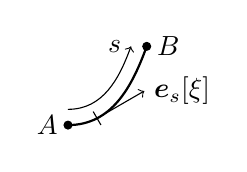
\begin{tikzpicture}
  \draw[thick] (0,0) to[out=0,in=250] coordinate[near start] (m) node[at start,left] {$A$} node[at end,right] {$B$} (1,1) ;
  \draw[->] (0,0.2) to[out=0,in=250] node[at end,left] {$s$} (0.8,1);
  \draw[|->] (m) -- +(30:0.7) node[at end,right] {$\to e_s[\xi]$};
  \draw[fill,black] (0,0) circle (0.05) (1,1) circle (0.05);
 \end{tikzpicture}
 \caption{Geometry and coordinate system for 2D (and axisymmetric)}
 \label{fig:extruded}
\end{figure}

The geometry is parameterized as
\begin{align}
 \to x &= \sum_{i=1}^n N_i[\xi]\to x_i
  = \um N \cdot \uv X
  = \underbrace{\begin{bmatrix}N_1 & 0 & \cdots\\ 0 & N_1 & \cdots \end{bmatrix}}_{2\times 2n}\cdot \underbrace{\begin{bmatrix}x_1\\y_1\\x_2\\y_2\\ \vdots\end{bmatrix}}_{2n\times 1}
\end{align}
so the divergence and integral can be rewritten by obtaining
\begin{gather}
 J \defeq \dderiv{s}{\xi} = \norm{\to x'}\\
 \to e_s \defeq \to x' J^{-1} = J^{-1}\sum_{i=1}^n N_i'[\xi] \to x_i\\
 \intd A = t \intd s = t J \intd \xi     \label{eq:intdA_2d}\\
 \to \nabla_s = \pderiv{}{s}\to e_s = \pderiv{}{\xi}\to e_s J^{-1}    \label{eq:nabla_s_2d}
\end{gather}
and for the tangent the following derivations are also usefull
\begin{align}
 \pderiv{\to x'}{\to x_i} &= N_i' \ts I & \pderiv{\to x'}{\uv X} &= \um N'\\
 \pderiv{J}{\to x_i} &= \to e_s \cdot \pderiv{\to x'}{\to x_i} = \to e_s N_i'  & \pderiv{J}{\uv X} &= \to e_s\cdot \um N' \\
 \pderiv{\to e_s}{\to x_i} &= (\ts I - \to e_s\otimes\to e_s)N_i' J^{-1} &  \pderiv{\to e_s}{\uv X} &= (\ts I - \to e_s\otimes \to e_s)\cdot \um N' J^{-1}
\end{align}

Plugging \eqref{eq:intdA_2d} and \eqref{eq:nabla_s_2d} into the integral in \eqref{eq:curvature}
\begin{align}
 \int_\Omega\to \nabla_s\cdot\to w\intd A &= t \int_{-1}^{1} \to w'\cdot \to e_s \intd\xi = \left( t \int_{-1}^1 \dderiv{\to w}{s} \cdot \to e_s\intd s\right)
\end{align}
and its tangent
\begin{align}
 \int_\Omega\to \nabla_s\cdot\to w\intd A \otimes \pderiv{}{\uv X}
 =&t \int_{-1}^{1} \left(\to w'\cdot \to e_s\right)\otimes \pderiv{}{\uv X}  \intd\xi\\
 =&t \int_{-1}^{1} \to w'\cdot \pderiv{\to e_s}{\uv X} \intd\xi\\
 =&t \int_{-1}^{1} \to w'\cdot \left(\ts I-\to e_s'\otimes\to e_s' \right)\cdot \um N' J^{-1} \intd\xi
\end{align}

% The boundary term is trivial
% \begin{gather}
%  \to m = \sign[\xi]\to e_s\\
%  \int_{\partial\Omega} \to w\cdot \to m\intd S = \to w \cdot\to m t = \sign[\xi]\to w \cdot \to e_s t
% \end{gather}
% and its tangent
% \begin{align}
%  \int_{\partial\Omega} \to w\cdot \to m\intd S\otimes \pderiv{}{\uv X} &= t \to w\cdot\pderiv{\to m}{\uv X}\\
%  &= \sign[\xi]t \to w\cdot\pderiv{\to e_s}{\uv X}\\
%  &= \sign[\xi]t \to w\cdot \left(\ts I-\to e_s\otimes\to e_s\right)\cdot \um N' J^{-1}
% \end{align}

The load vector becomes
\begin{align}
 \uv F &= -\gamma t \int_{-1}^{1} {\um N}'^\T\cdot \to e_s \intd\xi\\
       &= -\gamma t \int_{-1}^{1} \dderiv{{\um N}^\T}{s}\cdot \to e_s J \intd\xi \\
 \um K &= \gamma t \int_{-1}^{1} {\um N}'^\T\cdot \left(\ts I-\to e_s\otimes\to e_s\right)\cdot{\um N}' J^{-1} \intd\xi\\
       &=  \gamma t \int_{-1}^{1} \dderiv{\um N^\T}{s}\cdot \left(\ts I-\to e_s\otimes\to e_s\right)\cdot\dderiv{\um N}{s} J \intd\xi
\end{align}
% and the boundary term
% \begin{gather}
%  \uv F = \sign[\xi]\gamma t {\um N}^\T\cdot\to e_s\\
%  \um K = -\sign[\xi]\gamma t J^{-1} {\um N}^\T \cdot (\ts I - \to e_s\otimes \to e_s)\cdot {\um N}'
% \end{gather}

\subsection{Linear elements}
\begin{gather}
 \uv F_\linear = \gamma t L^{-1} \begin{bmatrix}x_2-x_1\\y_2-y_1\\x_1-x_2\\y_1-y_2\end{bmatrix}\\
 \um K_\linear = \gamma t L^{-1}\left(
	\begin{bmatrix}1&0&-1&0\\0&1&0&-1\\-1&0&1&0\\0&-1&0&1\end{bmatrix}-
	L^{-2}\begin{bmatrix}x_2-x_1\\y_2-y_1\\x_1-x_2\\y_1-y_2\end{bmatrix}\otimes\begin{bmatrix}x_2-x_1\\y_2-y_1\\x_1-x_2\\y_1-y_2\end{bmatrix}
  \right)
\end{gather}
% and for the boundary (boundary at $\to x_1$)
% \begin{gather}
%  \uv F_\linear = -\gamma t L^{-1} \begin{bmatrix}x_2-x_1\\y_2-y_1\\0\\0\end{bmatrix}\\
%  \um K_\linear = -\gamma t L^{-1} \left(\begin{bmatrix}1&0&-1&0\\0&1&0&-1\\0&0&0&0\\0&0&0&0\end{bmatrix} - L^{-2} \begin{bmatrix}x_2-x_1\\y_2-y_1\\0\\0\end{bmatrix}\otimes\begin{bmatrix}x_2-x_1\\y_2-y_1\\x_1-x_2\\y_2-y_1\end{bmatrix}2\right)\\
% \end{gather}

\section{Axisymmetric}
For brevity, the notation $(\bullet)' = \pderiv{\bullet}{\xi}$ or $(\bullet)' = \pderiv{\bullet}{\theta}$ is used for $f[\xi]$ and $f[\theta]$ respectively.

This part was more complicated than initially estimated.
I have consistently decomposed variables into $\ts Q$ to make this managable and also analytically calculating the integral over $\theta$.

With cylindrical coordinates $\to r = r\to e_r + z \to e_z$.
\begin{align}
 \to r &= \sum_i N_i[\xi]\to r_i = \um N\cdot \uv R\\
 x &= \cos[\theta] r\\
 y &= \sin[\theta] r\\
 z &= z\\
 \ts Q &= \begin{bmatrix}\cos[\theta] & 0\\ \sin[\theta] & 0\\ 0 & 1\end{bmatrix}\\
 \to x &= \ts Q[\theta] \cdot \to r[\xi]\\
 \to w &= \ts Q[\theta] \cdot \to v[\xi]\\
 \to m &= \ts Q[\theta] \cdot \to t[\xi]
\end{align}

Since we have a convenient orthogonality, we can treat $\xi$ and $\theta$ seperarely.
\begin{align}
 J_\xi &= \norm{\pderiv{\to x}{\xi}} = \norm{\ts Q \cdot \to r'} = \norm{\to r'}\\
 J_\theta &= \norm{\pderiv{\to x}{\theta}} = \norm{\ts Q' \cdot \to r} = r \\
 \intd A &= J_\xi J_\theta \intd \xi \intd \theta \\
 \to\nabla_s &= J_\xi^{-2} \pderiv{\to x}{\xi}\pderiv{}{\xi} + J_\theta^{-2} \pderiv{\to x}{\theta}\pderiv{}{\theta}
\end{align}
and for the tangent the following derivations are also usefull
\begin{align}
 \to e_s &\defeq \to r' J_\xi^{-1} & \uv D &\defeq \um N^\T \cdot \to e_s\\
 \uv A &\defeq {\um N}'^\T \cdot \to e_s & \uv B &\defeq \pderiv{r}{\uv R} = {\um N}^\T \cdot \begin{bmatrix}1\\0\end{bmatrix}\\
\end{align}
\begin{align}
 \pderiv{\to r'}{\to r_i} &= N_i' \ts I
	& \pderiv{\to r'}{\uv R} &= \um N'\\
 \pderiv{J_\xi}{\to r_i} &= \to e_s \cdot \pderiv{\to r'}{\to r_i} = \to e_s N_i'
	& \pderiv{J_\xi}{\uv R} &= \to e_s\cdot \um N' \\
 \pderiv{\to e_s}{\to r_i} &= (\ts I - \to e_s\otimes\to e_s)N_i' J_\xi^{-1}
	& \pderiv{\to e_s}{\uv R} &= (\ts I - \to e_s \otimes \to e_s )\cdot \um N' J_\xi^{-1}
\end{align}

Plugging this into \eqref{eq:curvature} to obtain
\begin{align}
 &\int_\Omega\to \nabla_s\cdot\to w\intd A\\
=&\int_{-1}^{1}\int_0^{2\pi}\left( J_\xi^{-2} \pderiv{\to x}{\xi}\cdot\pderiv{\to w}{\xi} +
                              J_\theta^{-2} \pderiv{\to x}{\theta}\cdot\pderiv{\to w}{\theta}
  \right) J_\xi J_\theta \intd \theta \intd \xi\\
=&\int_{-1}^{1}\int_0^{2\pi}\left(
	  J_\xi^{-2} (\ts Q^\T\cdot\ts Q):(\to r'\otimes \to v') +
	  J_\theta^{-2} ({\ts Q'}^\T\cdot\ts Q'):(\to r\otimes\to v)
  \right) J_\xi J_\theta \intd \theta \intd \xi\\
=&\int_{-1}^{1}\int_0^{2\pi}\left(
	  J_\xi^{-2} \ts I :(\to r'\otimes \to v') +
	  J_\theta^{-2} \begin{bmatrix}1&0\\0&0\end{bmatrix}:(\to r \otimes \to v)
  \right) J_\xi J_\theta \intd \theta \intd \xi\\
=&2\pi\int_{-1}^{1}\left( \to v' \cdot \to e_s r + \to v \cdot \begin{bmatrix}1\\0\end{bmatrix} J_\xi \right) \intd \xi\\
=&2\pi\int_{-1}^{1}\left( \dderiv{\to v}{s} \cdot \to e_s r + \to v \cdot \begin{bmatrix}1\\0\end{bmatrix} \right) \intd s
\end{align}
and its tangent
\begin{align}
 &\int_\Omega\to \nabla_s\cdot\to w\intd A \otimes \pderiv{}{\uv R} \\
 =& 2\pi \int_{-1}^{1} \left(
	\to v' \cdot \to e_s r + \to v\cdot \begin{bmatrix}1\\0\end{bmatrix} J_\xi
	\right)\otimes\pderiv{}{\uv R}\intd\xi\\
  =& 2\pi \int_{-1}^{1} \left(
	\to v' \cdot \to e_s \otimes \pderiv{r}{\uv R} + \to v'\cdot \pderiv{\to e_s}{\uv R} r + \to v\cdot \begin{bmatrix}1\\0\end{bmatrix}\otimes\pderiv{J_\xi}{\uv R}
	\right)\intd\xi\\
  =& 2\pi \int_{-1}^{1} \bigg(
	\to v' \cdot \to e_s \otimes\left(\begin{bmatrix}1&0\end{bmatrix}\cdot \um N\right) +
	\to v'\cdot (\ts I - \to e_s\otimes \to e_s)\cdot \um N' J_\xi^{-1} r
	+\to v\cdot \begin{bmatrix}1\\0\end{bmatrix}\otimes (\to e_s\cdot \um N')
	\bigg)\intd\xi
\end{align}

% The boundary term is computed as
% \begin{align}
%  \int_{\partial\Omega} \to w\cdot\to m\intd S &= \int_0^{2\pi} (\ts Q^\T\cdot \ts Q):(\to v\cdot\to t) r \intd \theta\\
%   &= 2\pi r \to v \cdot \to t = 2\pi\sign[\xi]r \to v\cdot \to e_s
% \end{align}
% and its tangent
% \begin{align}
%  \int_{\partial\Omega} \to w\cdot\to m\intd S \otimes \pderiv{}{\uv R} &= 2\pi\sign[\xi] (r \to v \cdot \to e_s)\otimes \pderiv{}{\uv R}\\
%   &= 2 \pi \sign[\xi]\left(\to v\cdot\to e_s\otimes\pderiv{r}{\uv R} + r \to v\cdot\pderiv{\to t}{\uv R}\right)\\
%   &= 2 \pi \sign[\xi]\left(\to v\cdot\to e_s\otimes\left(\begin{bmatrix}1&0\end{bmatrix}\cdot\um N\right) +  J_\xi^{-1} r \to v\cdot\left(\ts I-\to e_s\otimes\to e_s\right)\cdot \um N'\right)
% \end{align}

The load vector for an element is
\begin{gather}
 \uv F = -2\pi \gamma \int_{-1}^{1} \left(r{\um N}'^\T\cdot\to e_s + J_\xi{\um N}^\T\cdot\begin{bmatrix}1\\0\end{bmatrix}\right) \intd\xi
\end{gather}
\begin{multline}
 \um K = 2\pi \int_{-1}^{1} \bigg(
	{\um N}'^\T \cdot \to e_s \otimes {\um N}^\T\cdot \begin{bmatrix}1\\0\end{bmatrix} +\\
	{\um N}'^\T \cdot (\ts I - \to e_s\otimes \to e_s)\cdot {\um N}' J_\xi^{-1} r +
	{\um N}^\T \cdot \begin{bmatrix}1\\0\end{bmatrix}\otimes \to e_s\cdot {\um N}'
	\bigg)\intd\xi
\end{multline}
or
\begin{gather}
  \uv F = -2\pi \gamma \int_{-1}^{1} \left(r\uv A + J_\xi\uv B\right) \intd\xi\\
  \um K = 2\pi \int_{-1}^{1} \bigg(
	\uv A \otimes \uv B +
	\uv B\otimes \uv A +
	J_\xi^{-1} r({\um N}'^\T \cdot {\um N}' - \uv A\otimes \uv A)
	\bigg)\intd\xi
\end{gather}
% and for the boundary
% \begin{align}
%  \uv F &= 2\pi\gamma\sign[\xi] r {\uv N}^\T \cdot \to e_s = 2\pi\gamma\sign[\xi]\uv D\\
%  \um K &= -2 \pi \gamma \sign[\xi]\um N^\T\cdot\left(\to e_s\otimes\left(\um N^\T\cdot\begin{bmatrix}1\\0\end{bmatrix}\right) + J_\xi^{-1} r \left(\ts I-\to e_s\otimes\to e_s\right)\cdot \um N' \right)\\
%        &= -2 \pi \gamma \sign[\xi]\left(\uv D\otimes\uv B + J_\xi^{-1} r \left(\um N^\T\cdot\um N' -\uv D\otimes\uv A\right) \right)
% \end{align}

\subsection{Linear elements}

\begin{gather}
 \nonumber \hat{\uv A} = -L^{-1}\begin{bmatrix}r_2-r_1\\z_2-z_1\\r_1-r_2\\z_1-z_2\end{bmatrix}, \quad
 \hat{\uv B} = \begin{bmatrix}1\\0\\1\\0\end{bmatrix},\quad J_\xi = \frac12 L\\
 \uv F_\linear = -\pi \gamma \left((r_1+r_2)\hat{\uv A} + L\hat{\uv B}\right)\\
 \um K_\linear = \pi \gamma \left(
  \hat{\uv A}\otimes\uv B + \hat{\uv B}\otimes\hat{\uv A}
  + 2L^{-1} r \left(\begin{bmatrix}1&0&-1&0\\0&1&0&-1\\-1&0&1&0\\0&-1&0&1\end{bmatrix} - \hat{\uv A}\otimes\hat{\uv A}\right)
  \right)
\end{gather}
% and for boundary at $\to r_1$;
% \begin{gather}
%  \nonumber \uv B = \begin{bmatrix}1\\0\\0\\0\end{bmatrix}, \quad \uv D = L^{-1}\begin{bmatrix}r_2-r_1\\z_2-z_1\\0\\0\end{bmatrix}\\
%  \uv K_\linear = 2\pi \gamma\left(\uv D\otimes \uv B + L^{-1} r_1 \left(\begin{bmatrix}-1&0&1&0\\0&-1&0&1\\0&0&0&0\\0&0&0&0\end{bmatrix}- \uv D\otimes \hat{\uv A}\right)\right)\\
%  \uv F_\linear = -2\pi \gamma r_1 L^{-1} \begin{bmatrix}r_2-r_1\\z_2-z_1\\0\\0\end{bmatrix}
% \end{gather}

\section{General 3D}

Introducing another parameter $\zeta$ in order to obtain a nice mapping.
\begin{align}
 \to x[\xi,\eta,\zeta] &= (1+\zeta)\to n + \sum_i N_i[\xi,\eta]\to x_i  %= \to n + \um N \cdot \uv X\\
  %&= (1-\zeta) \begin{bmatrix}N_1 & 0 & 0 & N_2 & \cdots\\0&N_1&0&0&\cdots\\0&0&N_1&0&\cdots\end{bmatrix}\cdot\begin{bmatrix}x_1\\y_1\\z_1\\x_2\\\vdots\end{bmatrix}
\end{align}

\begin{gather}
 J \defeq \norm{\pderiv{\to x}{\xi} \times  \pderiv{\to x}{\eta}}\\
 \to n = \pderiv{\to x}{\xi} \times \pderiv{\to x}{\eta} J^{-1}\\
 \begin{bmatrix}\intd x\\ \intd y\\ \intd z\end{bmatrix} =
  \underbrace{\begin{bmatrix}\pderiv{x}{\xi} & \pderiv{x}{\eta} & \pderiv{x}{\zeta}\\
	  \pderiv{y}{\xi} & \pderiv{y}{\eta} & \pderiv{y}{\zeta}\\
	  \pderiv{z}{\xi} & \pderiv{z}{\eta} & \pderiv{z}{\zeta} \end{bmatrix}}_{\ts J}
  \cdot \begin{bmatrix}\intd \xi \\ \intd \eta \\ \intd \zeta\end{bmatrix}\\
  \ts J = \begin{bmatrix}\pderiv{x}{\xi} & \pderiv{x}{\eta} & n_1\\
	  \pderiv{y}{\xi} & \pderiv{y}{\eta} & n_2\\
	  \pderiv{z}{\xi} & \pderiv{z}{\eta} & n_3 \end{bmatrix}\\
 \to\nabla = \ts J^{-\T}\cdot\to\nabla_\xi\\
 \intd A = J \intd \xi \intd \eta 
\end{gather}

and we obtain
\begin{align}
 &\iint_\Omega\to \nabla_s\cdot\to w\intd A\\
=&\iint_\omega(\ts I-\to n\otimes\to n):(\to w\otimes \ts J^{-\T}\cdot\to\nabla_\xi)J\intd\xi\intd\eta\big|_{\zeta=0}\\
=&\iint_\omega(\ts I-\to n\otimes\to n):\left((\to w\otimes\to\nabla_\xi) \cdot\ts J^{-1}\right)J\intd\xi\intd\eta\big|_{\zeta=0}
%=&\iint_\omega((\ts I-\to n\otimes\to n)\cdot\ts J^{-\T}):(\to w\otimes\to\nabla_\xi)J\intd\xi\intd\eta\big|_{\zeta=0}\\
%=&\iint_\omega(\to w\otimes\to\nabla_\xi):((\ts I-\to n\otimes\to n)\cdot\ts J^{-\T})J\intd\xi\intd\eta\big|_{\zeta=0}
\end{align}

% And given an edge along $\xi$;
% \begin{align}
%  &\int_{\partial\Omega}\to w\cdot\to m\intd S\\
% =&\int_{\partial\omega}\to w\cdot\to m J_\xi \intd \xi\\
%  \hat{\to n} &= \to e_\xi \times \to e_\eta\\
%  \hat{\to m} &= \to e_\xi \times \hat{\to n} = \to e_\xi\times (\to e_\xi \times \to e_\eta)\\
%  \to m &= \hat{\to m}\norm{\to m}^{-1}
% \end{align}

It becomes a bit tricky to express the load vector nicely due to the appearance of a third order tensor, it will need to be reshaped.
After some rewriting the expression becomes
\begin{align}
 \hat{\uv N} &= \begin{bmatrix} N_1\\ N_2\\ \vdots\end{bmatrix}\\
 \hat{\um B} &= \ts J^{-\T}\cdot(\to\nabla_\xi\cdot(\hat{\uv N})^\T)\\
 \hat{\um F} &= \iint_\omega(\ts I-\to n \cdot \to n^\T)\cdot \hat{\um B} J\intd\xi\intd\eta\big|_{\zeta=0}\\
 \uv F &= \begin{bmatrix}\hat{\uv F}_{1:}\\\hat{\uv F}_{2:}\\\vdots\end{bmatrix}
\end{align}
% and along the boundary
% \begin{align}
%  \uv F &= \int_{\partial\omega}{\um N}^\T\cdot\to m J_\xi \intd \xi
% \end{align}


\section{General 3D alternative method}
\begin{align}
 \to x[\xi,\eta] = \sum_i N_i[\xi,\eta]\to x_i
\end{align}
\begin{gather}
 J \defeq \norm{\pderiv{\to x}{\xi} \times  \pderiv{\to x}{\eta}}\\
 \to n = \pderiv{\to x}{\xi} \times \pderiv{\to x}{\eta} J^{-1}\\
 \to e_s = \pderiv{\to x}{\xi}\norm{\pderiv{\to x}{\xi}}^{-1}\\
 \to e_t = -\to e_s\times \to n\\
 \begin{bmatrix}\intd x\\ \intd y\\ \intd z\end{bmatrix} =
  \underbrace{\begin{bmatrix}\pderiv{\to x}{\xi} & \pderiv{\to x}{\eta}
  \end{bmatrix}}_{\ts J''}
  \cdot \begin{bmatrix}\intd \xi \\ \intd \eta\end{bmatrix}\\
 \begin{bmatrix}\intd s\\ \intd t\end{bmatrix} =
  \underbrace{\begin{bmatrix} \to e_s^\T \\ \to e_t^\T
  \end{bmatrix}}_{\ts J'}
  \cdot \begin{bmatrix}\intd x \\ \intd y \\ \intd z\end{bmatrix}\\
 \intd A = J \intd \xi \intd \eta
\end{gather}

\begin{align}
 \to\nabla_s\cdot\to w &= \to\nabla_{st}\cdot\to w_{st} \\
 &= (\to w_{st}\otimes\to\nabla_{st}):\ts I \\
 &= \left(((\ts J'\cdot \to w) \otimes \to\nabla_{\xi\eta})\cdot \left(\ts J'\cdot\ts J''\right)^{-1}\right): \ts I\\
 &= \left((\to w\cdot (\ts J'^\T \otimes \to\nabla_{\xi\eta}) +\ts J'\cdot(\to w\otimes\to\nabla_{\xi\eta}) )\cdot \left(\ts J'\cdot\ts J''\right)^{-1}\right): \ts I
\end{align}
The gradient $\ts J'^\T \otimes\to\nabla_{\xi\eta}$ is bothersome.
\begin{align}
 \to e_s \otimes \to\nabla_{\xi\eta} = \text{ugh...}
\end{align}

Considering the special case of linear surfaces;
\begin{align}
  \to\nabla_s\cdot\to w &= \left(\ts J'\cdot(\to w\otimes\to\nabla_{\xi\eta})\cdot \left(\ts J'\cdot\ts J''\right)^{-1}\right): \ts I
\end{align}

\begin{align}
 &\iint_\Omega\to \nabla_s\cdot\to w\intd A\\
=&\iint_\omega \ts I:\left(\ts J'\cdot(\to w\otimes\to\nabla_{\xi\eta})\cdot \left(\ts J'\cdot\ts J''\right)^{-1}\right)J\intd\xi\intd\eta
\end{align}

\end{document}
